\documentclass[aspectratio=1610]{beamer}


\usepackage{listings}
\usepackage{tikz}
\usepackage{tikz-qtree}
\usepackage{subfig}
\def\addsquare#1{\tikz\node[draw]{#1};}
\def\addcircle#1{\tikz\node[draw,circle]{#1};}



\usepackage{xcolor}
\definecolor{pgreen}{rgb}{0,0.5,0}

\usetheme{Antibes}

\lstset{
    language=Java,
    showstringspaces=false,
    columns=flexible,
    basicstyle={\small\ttfamily},
    numbers=none,
    numberstyle=\tiny\color{gray},
    keywordstyle=\color{blue},
    commentstyle=\color{pgreen},
    stringstyle=\color{pgreen},
    breaklines=true,
    breakatwhitespace=true,
    tabsize=3,
    escapeinside={(*}{*)},
    aboveskip=-1em,
    belowskip=-1em,
}

%Information to be included in the title page:
\title{Incremental clone detection for IDEs using dynamic suffix arrays}
\author{Jakob Konrad Hansen}
\institute{University of Oslo}
\date{2023}



\begin{document}

\frame{\titlepage}

\begin{frame}
    \frametitle{Outline}
    \tableofcontents
\end{frame}

\section{Motivation and contribution}

\begin{frame}
\frametitle{Motivation}
\begin{itemize}
    \item Duplicated code is generally considered harmful to software quality
    \item Code clone detection, analysis and management is therefore important
    \item Incremental clone detection algorithms have not been thoroughly researched
    \item Incremental algorithms are useful in use-cases such as in IDEs
\end{itemize}
\end{frame}

\begin{frame}
\frametitle{Our contribution}
\begin{itemize}
    \item CCDetect-LSP: An incremental clone detection tool for IDEs
    \item Uses a novel application of dynamic extended suffix arrays for clone detection
    \item Language- and IDE agnostic via Tree-sitter and LSP
\end{itemize}
\end{frame}

\section{Background}

\subsection{Code clone theory}

\begin{frame}
    \frametitle{Code clones}

    \begin{definition}[Code snippet]
        A code snippet is a piece of contiguous source code in a larger software system.
    \end{definition}

    \begin{definition}[Code clone]
        A code clone is a code snippet which is equal or similar to another code snippet. The two
        code snippets are both code clones, and together they form a clone pair.
        Similarity is determined by some metric such as number of equal lines of code.
    \end{definition}
\end{frame}

\begin{frame}
	\frametitle{Clone types}
	\begin{itemize}
		\item Code clones are classified into four types
		      \begin{itemize}
			      \item Type-1: Syntactically identical
			      \item Type-2: Structurally identical
			      \item Type-3: Structurally similar
			      \item Type-4: Functionally similar (generally)
		      \end{itemize}
	\end{itemize}
\end{frame}


\begin{frame}[fragile]
	\frametitle{Clone type examples: type-1 and type-2}
    \begin{figure}[t]
		\begin{center}
			\begin{tabular}{c | c}
				\begin{lstlisting}
for (int i = 0; i < 10;   i++) {
    print(i);
}
\end{lstlisting} &
				\begin{lstlisting}
for (int i = 0; i < 10; i++) {
    // A comment

    print(i);
}
            \end{lstlisting}
			\end{tabular}
		\end{center}
        \caption{Type-1 clone pair}
    \end{figure}
    \begin{figure}[t]
        	\begin{center}
        \begin{tabular}{p{6cm} | p{6cm}}
\begin{lstlisting}
for (int i = 0; i < 10; i++) {
    print(i);
}
\end{lstlisting} & \begin{lstlisting}
for (int (*\textbf j*) = (*\textbf 5*); (*\textbf j*) < (*\textbf{20}*); (*\textbf j++*)) {
    print((*\textbf j*));
}
\end{lstlisting}
		\end{tabular}
	\end{center}

        \caption{Type-2 clone pair}
    \end{figure}

\end{frame}


\begin{frame}[fragile]
	\frametitle{Clone type examples: type-3 and type-4}
    \vspace{0.5cm}
	\begin{figure}[t]
		\begin{center}
			\begin{tabular}{p{6cm} | p{6cm}}
				\begin{lstlisting}
for (int i = 0; i < 10; i++) {
    print(i);
}\end{lstlisting} &
				\begin{lstlisting}
for (int i = 0; i < 10; i++) {
    print(i);
    print(i*2);
}\end{lstlisting}
			\end{tabular}
		\end{center}
		\caption{Type-3 clone pair}
		\label{fig:type3clone}
	\end{figure}
    \vspace{-0.5cm}

	\begin{figure}[t]
		\begin{center}
			\begin{tabular}{r | p{6.5cm}}
				\hspace{3.2cm}\begin{lstlisting}
print((n*(n-1))/2)
\end{lstlisting} &
				\begin{lstlisting}
int sum = 0;
for (int i = 0; i < n; i++) {
    for (int j = i+1; j < n; j++) {
        sum++;
    }
}
print(sum);
            \end{lstlisting}
			\end{tabular}
		\end{center}
		\caption{Type-4 clone pair}
		\label{fig:type4clone}
	\end{figure}
\end{frame}

\begin{frame}{Clone detection}
    \begin{figure}
        \begin{center}
            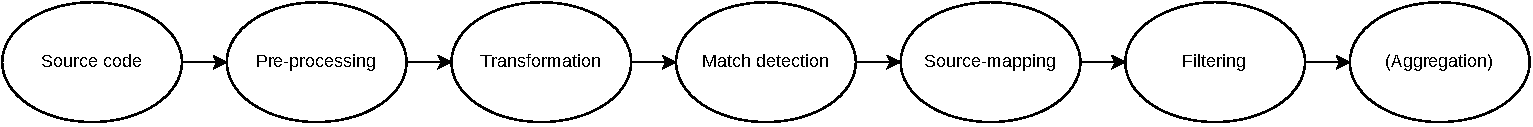
\includegraphics[width=0.95\textwidth]{figures/detectionphases.drawio.pdf}
        \end{center}
    \end{figure}
\end{frame}

\begin{frame}{Clone matching techniques}
    \begin{itemize}
        \item Text-based detection
            \begin{itemize}
                \item Match based on raw source code
            \end{itemize}
        \item Token-based detection
            \begin{itemize}
                \item Match based on tokens
            \end{itemize}
        \item Syntactic detection
            \begin{itemize}
                \item Match based on AST
            \end{itemize}
        \item Hybrid detection
            \begin{itemize}
                \item Combine multiple approaches
            \end{itemize}
    \end{itemize}
\end{frame}


\subsection{Preliminary algorithms and data structures}
\begin{frame}{Parsing and incremental parsing}
    \begin{figure}
        \begin{center}
            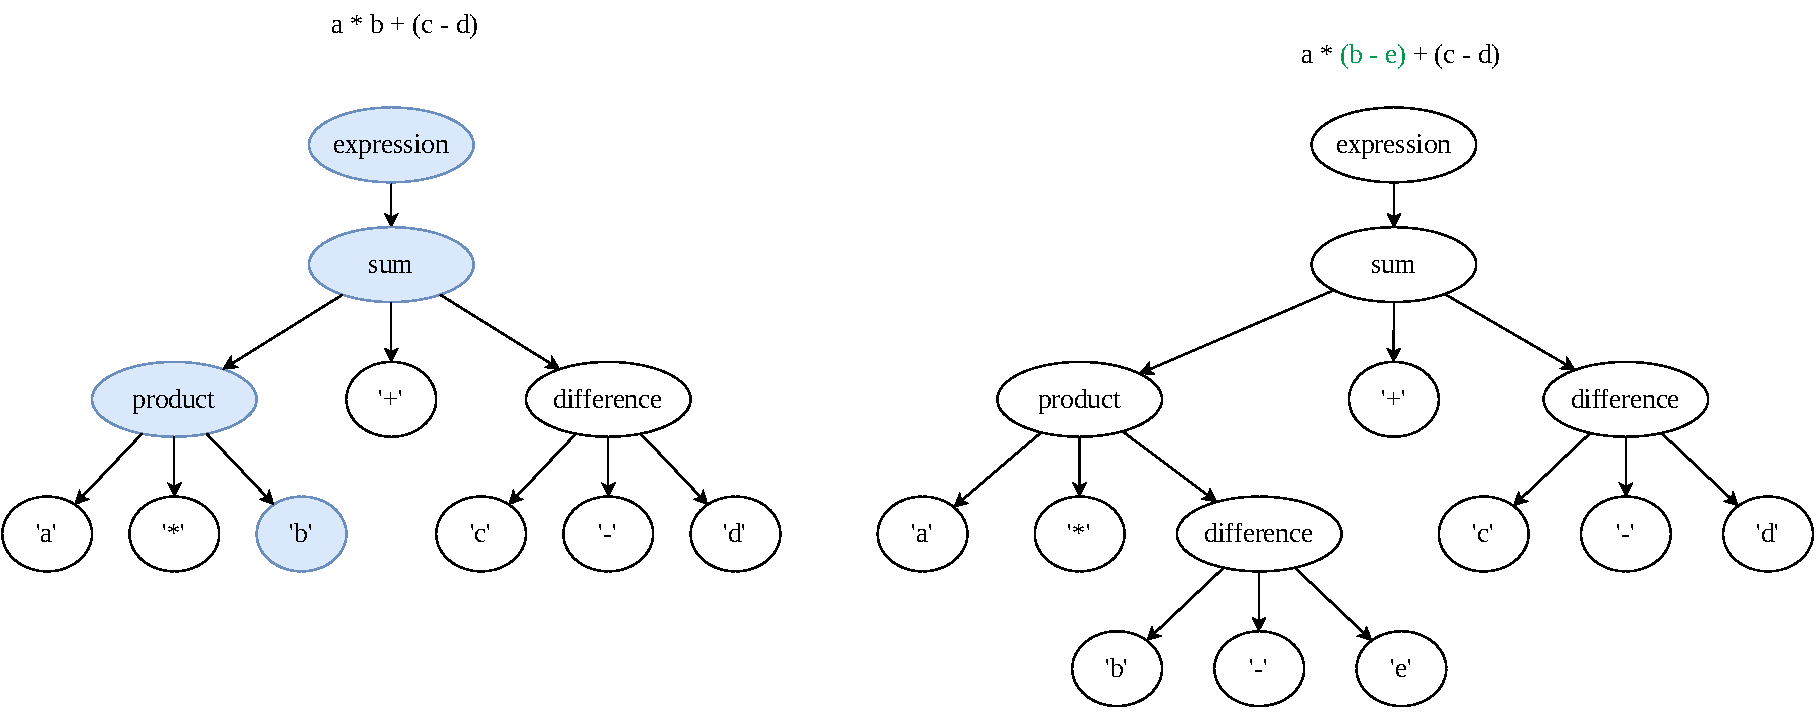
\includegraphics[width=0.95\textwidth]{figures/incrementalparsing.drawio.pdf}
        \end{center}
    \end{figure}
\end{frame}

\begin{frame}{Suffix tree}
	\begin{figure}
		\begin{center}
			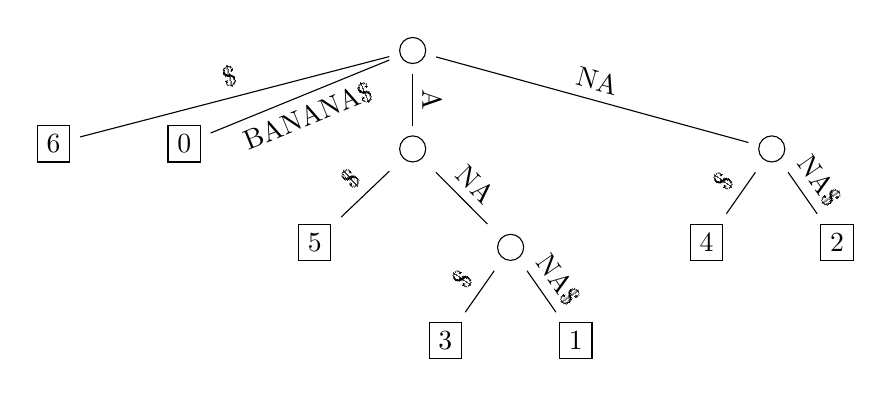
\begin{tikzpicture}[every tree node,
					level distance=1.25cm,sibling distance=1cm,
					edge from parent path={(\tikzparentnode) -- (\tikzchildnode)}]
				\Tree
				[.\addcircle{}
				\edge node[midway, above, sloped] {\$};
				[.\addsquare{6} ]
				\edge node[midway, below, sloped] {BANANA\$};
				[.\addsquare{0} ]
				\edge node[midway, above, sloped] {A};
				[.\addcircle{}
				\edge node[midway, above, sloped] {\$};
				[.\addsquare{5} ]
				\edge node[midway, above, sloped] {NA};
				[.\addcircle{}
				\edge node[midway, above, sloped] {\$};
				[.\addsquare{3} ]
				\edge node[midway, above, sloped] {NA\$};
				[.\addsquare{1} ]
				]
				]
				\edge node[midway, above, sloped] {NA};
				[.\addcircle{}
				\edge node[midway, above, sloped] {\$};
				[.\addsquare{4} ]
				\edge node[midway, above, sloped] {NA\$};
				[.\addsquare{2} ]
				]
				]
			\end{tikzpicture}
			\caption{Suffix tree for $S=\text{BANANA\$}$}
			\label{fig:suffixtree}
		\end{center}
	\end{figure}
\end{frame}

\begin{frame}{Suffix array}
	\begin{table}
		\begin{center}
			\subfloat[Suffixes]{
				\begin{tabular}{c | l }
					Index & Suffix   \\
					\hline
					0     & BANANA\$ \\
					1     & ANANA\$  \\
					2     & NANA\$   \\
					3     & ANA\$    \\
					4     & NA\$     \\
					5     & A\$      \\
					6     & \$       \\
				\end{tabular}}
			\hspace{1cm}
			\subfloat[Sorted suffixes]{\begin{tabular}{c | l}
					Index & Suffix   \\
					\hline
					6     & \$       \\
					5     & A\$      \\
					3     & ANA\$    \\
					1     & ANANA\$  \\
					0     & BANANA\$ \\
					4     & NA\$     \\
					2     & NANA\$   \\
				\end{tabular}}
			\hspace{1cm}
			\subfloat[SA, ISA and LCP]{\begin{tabular}{c | c | c | c}
					Index & SA & ISA & LCP \\
					\hline
					0     & 6  & 4   & 0   \\
					1     & 5  & 3   & 0   \\
					2     & 3  & 6   & 1   \\
					3     & 1  & 2   & 3   \\
					4     & 0  & 5   & 0   \\
					5     & 4  & 1   & 0   \\
					6     & 2  & 0   & 2   \\
				\end{tabular}}
		\end{center}
	\end{table}

\end{frame}
    
\begin{frame}{Burrows-Wheeler transform}
    \begin{table}
	\begin{center}
        \subfloat[Cyclic shifts]{
		\begin{tabular}{c | l }
			Index & CS   \\
			\hline
			0     & BANANA\$ \\
			1     & ANANA\$B \\
			2     & NANA\$BA \\
			3     & ANA\$BAN \\
			4     & NA\$BANA \\
			5     & A\$BANAN \\
			6     & \$BANANA \\
    \end{tabular}}
		\hspace{0.25cm}
        \subfloat[Sorted cyclic shifts and BWT]{\begin{tabular}{c | l}
			Index & CS   \\
			\hline
            6     & \$BANAN\textbf{A} \\
            5     & A\$BANA\textbf{N} \\
			3     & ANA\$BA\textbf{N} \\
			1     & ANANA\$\textbf{B} \\
			0     & BANANA\textbf{\$} \\
			4     & NA\$BAN\textbf{A} \\
			2     & NANA\$B\textbf{A} \\
    \end{tabular}}
		\hspace{0.25cm}
        \subfloat[LF function]{\begin{tabular}{c | l}
			L & F   \\
			\hline
            0     & $Rank_A(0) + C[A] = 0 + 1 = 1$\\
            1     & $Rank_N(1) + C[N] = 0 + 5 = 5$ \\
			2     & $Rank_N(2) + C[N] = 1 + 5 = 6$ \\
			3     & $Rank_B(3) + C[B] = 0 + 4 = 4$ \\
            4     & $Rank_{\$}(4) + C[\$] = 0 + 0 = 0$ \\
			5     & $Rank_A(5) + C[A] = 1 + 1 = 2$ \\
			6     & $Rank_A(6) + C[A] = 2 + 1 = 3$ \\
    \end{tabular}}
    \caption{S = BANANA\$, BWT = ANNB\$AA}
    \label{table:bwt}
	\end{center}
\end{table}
\end{frame}

\section{Implementation}

\subsection{Features}

\begin{frame}{CCDetect-LSP features}
	\begin{itemize}
		\item CCDetect-LSP is implemented as an LSP server
            \begin{itemize}
                \item List clones
                \item Display clones inline with code
                \item Jump between matching clones
                \item Incremental updates on each edit
            \end{itemize}
	\end{itemize}
\end{frame}

\subsection{Initial clone detection}

\begin{frame}{Implementation: Initial clone detection}
    \begin{itemize}
        \item Algorithm which initially detects type-1 and optionally type-2 clones
        \item Pipeline of 5 phases, returns a list of clones
        \item Uses an extended suffix array for match detection
        \item Starting point: Assume documents are indexed
    \end{itemize}
\end{frame}

\begin{frame}{Detection algorithm overview}
    \begin{figure}
        \begin{center}
            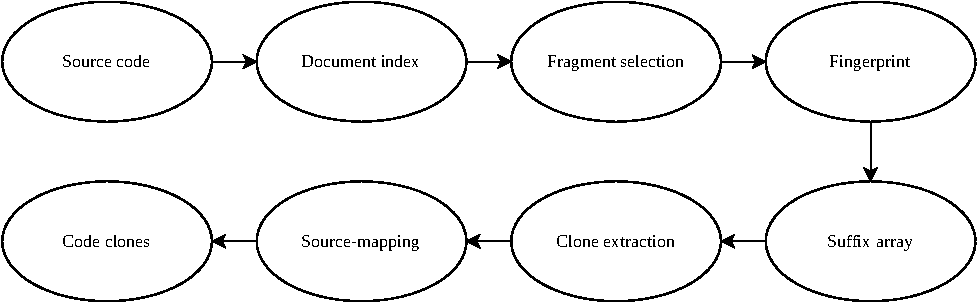
\includegraphics[width=0.95\textwidth]{figures/phases_all.drawio.pdf}
        \end{center}
        \caption{Overview of detection algorithm phases}
    \end{figure}
\end{frame}

\begin{frame}{Phase 1: Fragment selection}
    \begin{itemize}
        \item Parse files using Tree-sitter
        \item Use a configurable Tree-sitter query to ``capture'' nodes
        \item Extract and store the tokens of captured nodes
    \end{itemize}
\end{frame}

\begin{frame}{Phase 2: Fingerprinting}
    \begin{itemize}
        \item Consistently hash each token value with an increasing integer counter
        \item Store the fingerprint of each fragment in the document index
        \item For type-2 detection, hash the token type instead
    \end{itemize}
\end{frame}

\begin{frame}{Phase 2: Fingerprinting}
    \begin{itemize}
        \item Example here
    \end{itemize}
\end{frame}

\begin{frame}{Phase 3: Suffix array construction}
    \begin{itemize}
        \item Concatenate the fingerprints of each document in the index
        \item Construct SA, ISA and LCP array of the full fingerprint
        \item Uses ``Induced sorting variable-length LMS-substrings'' (SA-IS) algorithm
    \end{itemize}
\end{frame}

\begin{frame}{Phase 4: Clone extraction}
    
\end{frame}

\begin{frame}{Phase 5: Source-mapping}
    
\end{frame}


\subsection{Incremental clone detection}
\begin{frame}{Implementation: Incremental clone detection}
\end{frame}

\section{Evaluation}
\begin{frame}{Results}
\end{frame}

\section{Discussion}
\begin{frame}{Discussion}
\end{frame}

\section{Conclusion}
\begin{frame}{Conclusion}
	\begin{itemize}
		\item Why do people use clone detection tools?
	\end{itemize}
\end{frame}

\section{Demo?}

\begin{frame}{Demo}
    \begin{itemize}
        \item Demo!
    \end{itemize}
\end{frame}

\begin{frame}{Implementation: LSP architecture and functionality}
    \begin{figure}
        \begin{center}
            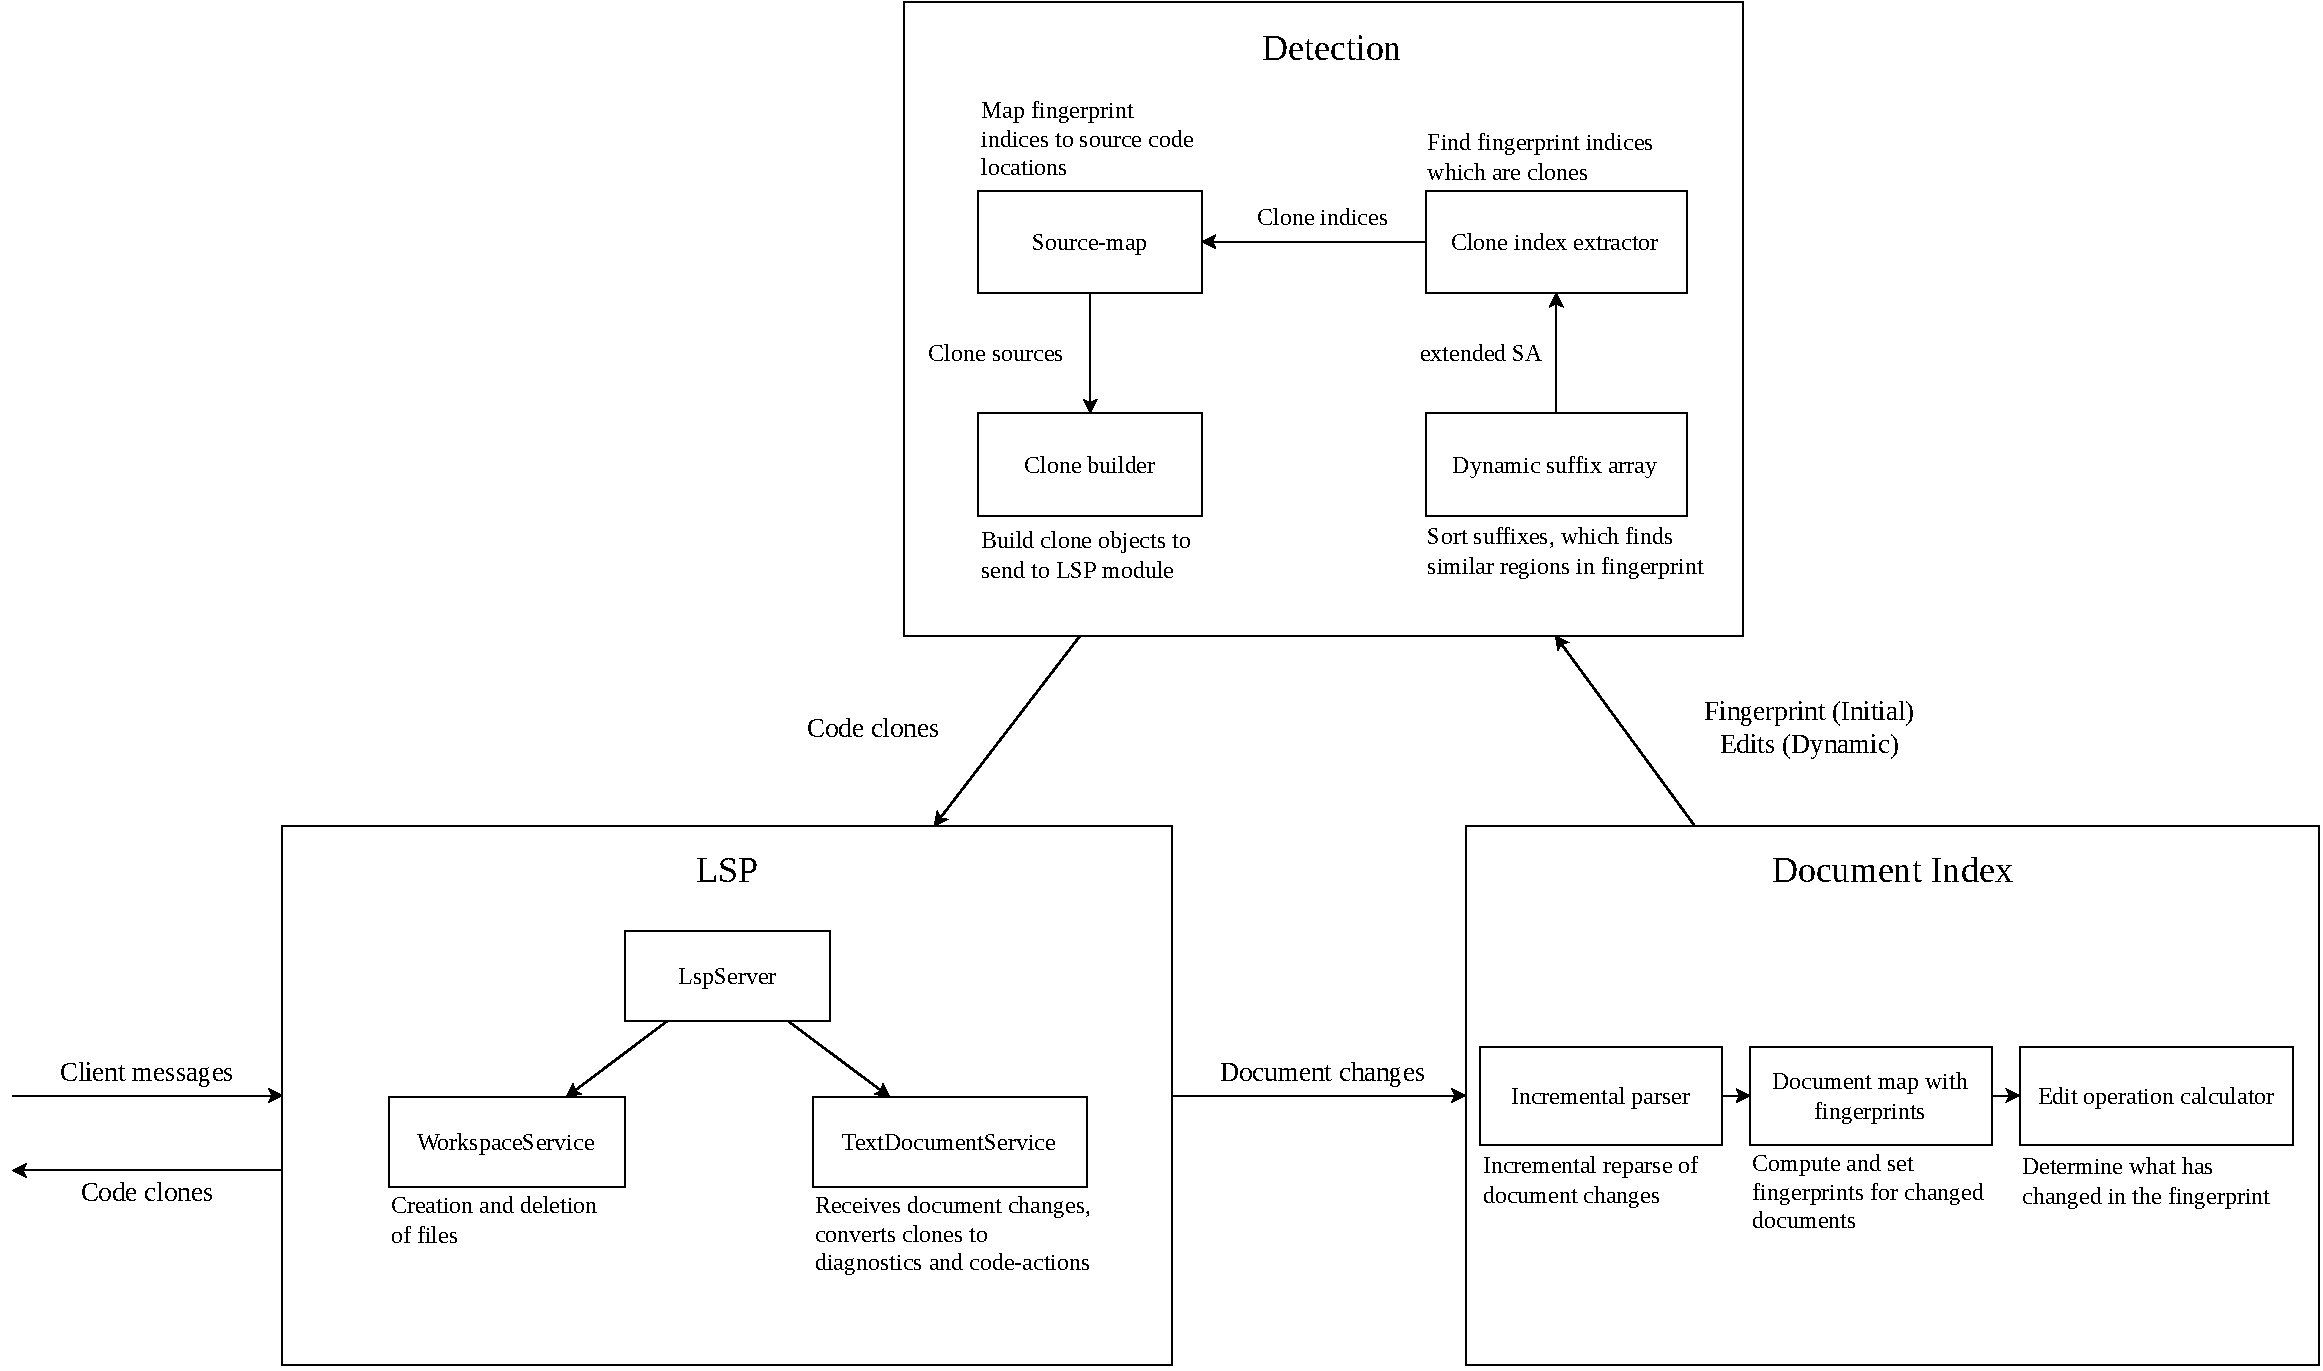
\includegraphics[width=0.7\textwidth]{figures/architecture.drawio.pdf}
        \end{center}
        \caption{Architecture of CCDetect-LSP}
    \end{figure}
\end{frame}

\begin{frame}{LSP}
    \begin{figure}
        \begin{center}
            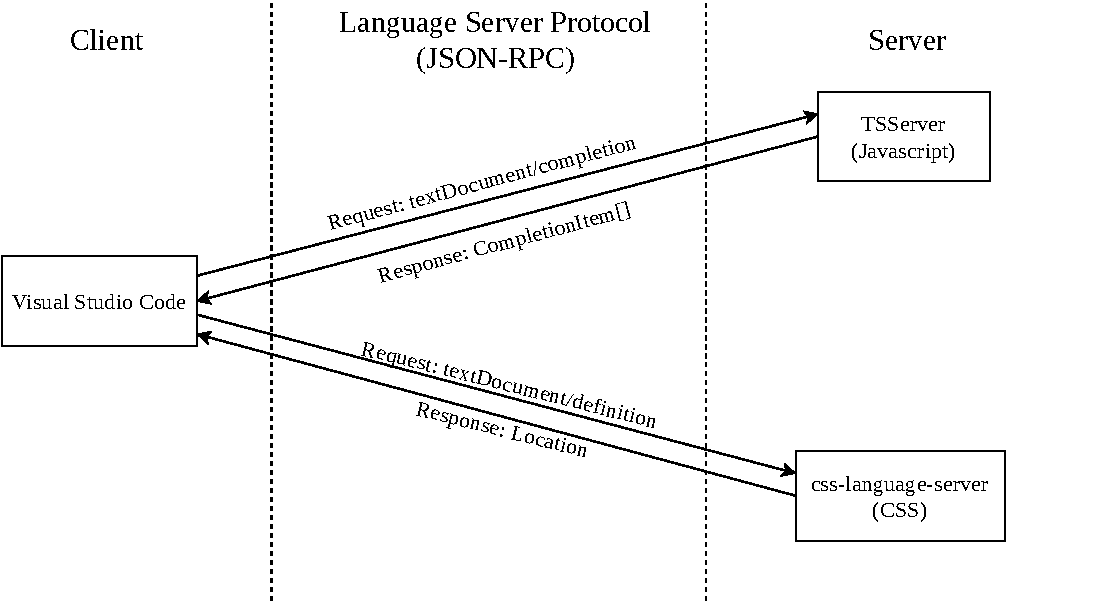
\includegraphics[width=0.7\textwidth]{figures/lspcommunication.drawio.pdf}
        \end{center}
        \caption{Example LSP server communication}
    \end{figure}
\end{frame}

\end{document}
